\documentclass[10pt]{extarticle}

% Lingua e matematica
\usepackage[english]{babel}
\usepackage{amsmath,amssymb,amsthm}

% Grafica e tabelle
\usepackage{graphicx}
\usepackage{subcaption}
\usepackage{float}
\usepackage{booktabs}
\usepackage{multirow}
\usepackage{siunitx}

% Codice (opzionale)
\usepackage{listings}
\usepackage{xcolor}
\definecolor{codegreen}{rgb}{0,0.6,0}
\definecolor{codegray}{rgb}{0.5,0.5,0.5}
\definecolor{codepurple}{rgb}{0.58,0,0.82}
\definecolor{backcolour}{rgb}{0.98,0.98,0.98}
\lstdefinestyle{mystyle}{
  backgroundcolor=\color{backcolour},
  commentstyle=\color{codegreen},
  keywordstyle=\color{magenta},
  numberstyle=\tiny\color{codegray},
  stringstyle=\color{codepurple},
  basicstyle=\ttfamily\footnotesize,
  breaklines=true, keepspaces=true, numbers=none, tabsize=2
}
\lstset{style=mystyle}

% Margini
\usepackage[margin=0.6in]{geometry}
\usepackage{ragged2e}
\usepackage{enumitem}
\usepackage[utf8]{inputenc} % per caratteri UTF-8 nei .tex e nel .bib
\usepackage{csquotes}       % consigliato da biblatex (evita warning e parse strani)



% Bibliografia (biblatex + biber)
\usepackage[backend=biber,style=ieee]{biblatex}
\addbibresource{references.bib}

% TOC: includi anche \paragraph e numerali
\setcounter{secnumdepth}{2}
\setcounter{tocdepth}{2}

% Hyperref (sempre *dopo* gli altri pacchetti)
\usepackage[colorlinks=true,linkcolor=blue,citecolor=teal,urlcolor=magenta]{hyperref}


\begin{document}

% Custom header without a separate titlepage
\noindent
\begin{minipage}{0.3\textwidth}
    
\includegraphics[width=1.3\linewidth]{Figures/polito_logo_2021_blu.jpg}
\end{minipage}
\hfill
\begin{minipage}{0.68\textwidth}
    \raggedleft
    {\LARGE \textbf{Politecnico di Torino}}\\[0.2cm]
    {\large Master's Degree in Mathematical Engineering}\\[0.7cm]
    {\large \textbf{Material for Thesis}}\\[0.2cm]
    {\large 3-- About GSE67919's Application }\\[0.7cm]
    \begin{tabular}{rl}
        Elisabetta Roviera & \texttt{s328422} \\
    \end{tabular}
\end{minipage}

\vspace{1cm}
\hrule
\vspace{0.5cm}

\tableofcontents

\vspace{0.5cm}
\hrule
\vspace{1cm}


% Main content begins here, on the same page
\justifying

\paragraph{Note} 
The papers summarized in this report represent the main references related to the GSE69914 dataset and to the preliminary filtering and quality control of CpG sites performed prior to the core analyses. These studies provide the methodological and technical background necessary to understand probe reliability, normalization strategies, and preprocessing pipelines applied to Illumina HumanMethylation450 data. Additional references may be integrated in the future to refine specific analytical steps. For a complete understanding of the concepts and results discussed, please refer to the original publications cited in the bibliography of this document.

\section{Discovery of cross-reactive probes and polymorphic CpGs in the Illumina Infinium HumanMethylation450 microarray}

\paragraph{Keywords}
DNA methylation, CpG sites, Illumina 450K array, cross-reactive probes, polymorphic CpGs, SNPs, microarray reliability, sex-associated methylation, probe specificity~\cite{chen2013crossreactive}

\paragraph{Cross-reactive probes}
Approximately 6\% of the probes on the Illumina HumanMethylation450 array hybridize to multiple genomic regions with high sequence similarity ($\geq$94\%). These cross-reactive probes can generate spurious methylation signals, particularly in autosomal sites that co-hybridize with sex chromosomes. As a result, apparent sex-associated methylation differences may arise as technical artifacts rather than biological effects. Probes showing $\geq$47 matched bases to unintended genomic loci were classified as cross-reactive and should be excluded from downstream analyses.

\paragraph{Polymorphic CpGs}
About 13.8\% of probes overlap known single nucleotide polymorphisms (SNPs), affecting either the cytosine, guanine, or the base immediately preceding the CpG site. These polymorphic CpGs reflect underlying genetic variation instead of true methylation differences. Their inclusion can distort methylation quantitative trait loci (mQTL) analyses or group comparisons if genotype effects are not accounted for.

\paragraph{Implications for preprocessing}
Cross-reactive and polymorphic probes can introduce false biological associations and reduce reproducibility. For accurate methylation profiling, these probes must be filtered before normalization and statistical modeling. The lists provided by Chen et al. are now widely used as reference sets in preprocessing pipelines for datasets such as GSE69914.

\paragraph{Impact on Illumina 450K analysis}
This study established essential quality-control guidelines for HumanMethylation450 data. By identifying unreliable probes and defining sequence-based exclusion criteria, it laid the groundwork for standardized preprocessing workflows and for accurate biological interpretation of CpG methylation patterns.

\section{The integrative epigenomic-transcriptomic landscape of ER-positive breast cancer}

\paragraph{Keywords}
ER-positive breast cancer, DNA methylation, RNA-Seq, Illumina 450K, TCGA, FEM algorithm, iCluster, luminal-A/B subtypes, WNT signaling, TGF-beta pathway, differential methylation, network analysis~\cite{gao2015integrative}.

\paragraph{Study design and rationale}
The study integrated DNA methylation (Illumina 450K) and RNA-Seq data from 724 estrogen receptor–positive (ER+) breast cancers and 111 normal adjacent tissues from the TCGA dataset to define functional epigenetic alterations driving tumor subtypes. Using the \textbf{Functional Epigenetic Modules (FEM)} algorithm, the authors identified network-level hotspots of coordinated DNA methylation and gene-expression changes, focusing on how epigenetic regulation contributes to luminal-A and luminal-B classification.

\paragraph{Data preprocessing and integration}
Methylation data (395,775 CpGs) and RNA-Seq expression data (20,531 genes) were preprocessed using standard Illumina and \texttt{limma} normalization procedures. Genes were assigned promoter methylation values by averaging probes mapping to TSS200 or first exon regions; if unavailable, TSS1500 was used. Probes mapping to gene bodies were excluded to focus on regulatory methylation. Empirical Bayes statistics (\texttt{limma}) were computed for differential methylation and expression between normal and ER+ samples. These gene-level statistics were integrated into a protein–protein interaction (PPI) network derived from high-confidence interactomes.

\paragraph{The FEM algorithm}
Each PPI edge connecting genes \( g, h \) was weighted using an anti-correlation rule combining differential methylation (\( t^D_g \)) and expression (\( t^R_g \)):
\[
w_{gh} = \frac{1}{2} \left( t^I_g + t^I_h \right), \quad 
t^I_g = H(t^D_g)H(-t^R_g) + H(-t^D_g)H(t^R_g),
\]
where \(H(x)\) is the Heaviside step function.
The network was scanned for dense subnetworks (“modules”) maximizing average edge weight (local modularity) using a spin-glass community detection algorithm. Significant modules were validated via permutation tests and comparison to null networks.

\paragraph{Identified FEM modules}
Nine significant FEMs were detected, encompassing 257 unique genes (146 both differentially methylated and expressed, 99 showing anti-correlation). Each FEM corresponded to a biologically meaningful hotspot. Representative examples include:
\begin{itemize}[label=-]
\item \textbf{CAV1 module} – enriched in WNT signaling genes (e.g., \textit{WIF1}, \textit{WNT3A}, \textit{SFRP1}), showing promoter hypermethylation and transcriptional repression.
\item \textbf{FSTL1 module} – enriched in TGF-$\beta$/BMP signaling members (\textit{BMP2}, \textit{BMP6}, \textit{BMP7}, \textit{TGFB2}), with widespread hypermethylation of tumor suppressor components.
\item \textbf{CCL11 and LEP modules} – involved in chemokine and GPCR signaling, with hypomethylation and overexpression consistent with enhanced metastatic potential.
\item \textbf{PROC and MME modules} – linked to coagulation and endothelin pathways, known to support tumor cell migration and proliferation.
\end{itemize}

\paragraph{Validation and reproducibility}
Independent datasets (Germany: 254 ER+ and 49 normal tissues; Yu: 110 ER+ and 13 normals) confirmed the FEM hotspots by network modularity and directional consistency of methylation and expression \(t\)-statistics. Four of nine FEMs achieved significant validation (\(p<0.05\)), and all showed concordant differential patterns across cohorts. Methylation datasets included GEO accession GSE69914, confirming overlap with the platform used in the present thesis.

\paragraph{Integrative clustering (iCluster analysis)}
Joint latent variable modeling (\texttt{iCluster}) of 463 ER+ TCGA tumors with matched DNAm and mRNA data (FEM genes only) identified exactly two integrative clusters (\(k=2\)), strongly corresponding to luminal-A and luminal-B subtypes (Fisher test \(p < 10^{-10}\)).  
Luminal-B tumors exhibited significantly higher deviation scores from the normal reference in both methylation and expression, indicating stronger epigenetic deregulation rather than distinct pathway activation. A similar two-cluster structure persisted when extending the input to 4311 anti-correlated genes genome-wide, confirming the homogeneity of ER+ epigenetic architecture.

\paragraph{Deviation scoring and prognosis}
A per-sample FEM deviation score quantified the combined distance (Z-normalized) of each gene’s methylation and expression from the normal baseline:
\[
FEM_s = \frac{1}{m} \sum_{g=1}^{m} |Z^D_{gs} - \alpha Z^R_{gs}|,
\]
with \(\alpha = \sigma_Z^D / \sigma_Z^R\) scaling data-type variance.  
Luminal-B samples displayed higher deviation scores than luminal-A in all modules (\(p<10^{-5}\)). Prognostic modeling (Cox regression across TCGA, METABRIC, and Fleischer datasets) showed that higher FEM scores and cluster membership were associated with worse survival (meta-analysis \(p=0.013\) for DNAm-based classifier).

\paragraph{Coordination of methylation–expression changes}
Unlike copy number alterations, methylation changes across FEM genes were found to be \textbf{coordinated}, not mutually exclusive, within tumors. Binary matrices of gene activation (1) vs normal-like (0) states revealed significantly smaller Manhattan distances between FEM genes than expected under random permutation (\(p<0.001\)), demonstrating intra-tumor coherence of epigenetic deregulation.

\paragraph{Biological interpretation}
ER+ luminal-A and luminal-B cancers share the same deregulated epigenetic pathways, dominated by silencing of WNT and BMP/TGF-$beta$ signaling antagonists. Luminal-B tumors exhibit larger magnitude deviations—reflecting stronger pathway repression, higher proliferation (correlation of FEM score with PCNA \(r \approx 0.38\)), and worse clinical outcomes.  
Epigenetic silencing of \textit{WIF1}, \textit{SFRP1}, and \textit{FSTL1} likely enhances WNT/TGF-$\beta$ signaling activity, promoting cell self-renewal and EMT. Additional deregulation in chemokine and endothelin pathways underscores a coordinated shift toward proliferative and migratory phenotypes.

\paragraph{Summary of methodology for replication}
To reproduce the FEM-based integration in a 450K dataset (e.g., GSE69914):
\begin{enumerate}
\item Preprocess IDATs (filter detection $p>0.01$; impute missing values $k=5$; exclude body probes).
\item Compute per-gene differential methylation and expression using empirical Bayes (\texttt{limma}).
\item Build a weighted PPI using the Heaviside anti-correlation rule.
\item Apply spin-glass modularity optimization to extract FEMs; validate with 1000 permutations.
\item Perform pathway enrichment (MSigDB) and compute per-sample FEM deviation scores.
\item Integrate FEM DNAm and mRNA matrices via \texttt{iCluster} to identify subtypes ($k=2$).
\item Optionally, compare FEM-derived subtypes to luminal-A/B and assess prognostic value.
\end{enumerate}

\paragraph{Conclusion}
The integrative analysis reveals that ER+ breast cancers form two principal epigenetic clusters corresponding to luminal-A and luminal-B phenotypes. Both subtypes share deregulated WNT and TGF-$\beta$/BMP networks, but luminal-B tumors exhibit greater magnitude of methylation-driven transcriptional repression. The study establishes a reproducible, network-based framework for identifying epigenetic driver modules and for quantifying coordinated methylation–expression shifts in large-scale 450K datasets.

\begin{figure}[h]
    \centering
    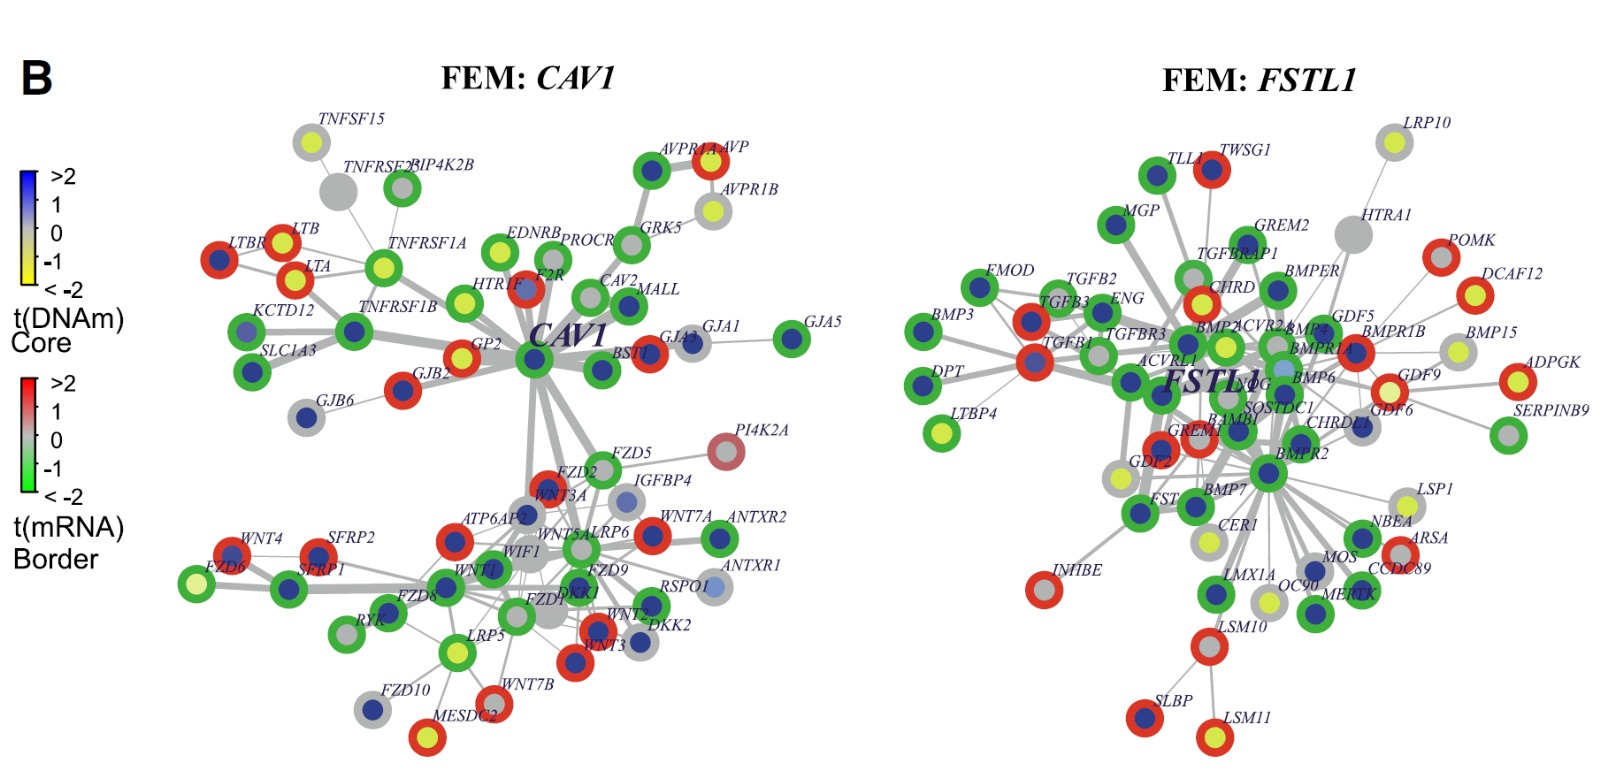
\includegraphics[width=0.5\textwidth]{Figures/Examples of two FEMs centred around seed genes CAV1 and FSTL1 in ER+ breast cancer.jpg} % o .png, .pdf, .eps...
    \caption{Examples of two FEMs centred around seed genes CAV1 and FSTL1 in ER+ breast cancer.}
    \label{fig:FEMs}
\end{figure}


\section{DNA methylation outliers in normal breast tissue identify field defects that are enriched in cancer}


\paragraph{Keywords}
Breast cancer, field defects, DNA methylation, Illumina 450K, epigenetic outliers, differential variability, iEVORA, DVMCs, adipose deconvolution, WNT signaling, GSE69914~\cite{teschendorff2016fielddefects}.

\paragraph{Study design and cohorts}
Genome-wide DNA methylation (DNAm) was profiled using the Illumina HumanMethylation450 BeadChip in a total of 407 breast tissue samples. The core discovery set included: (i) 50 normal/benign breast tissue samples from cancer-free women, (ii) 42 normal breast tissue samples adjacent to invasive breast cancers from the same patients (``normal-adjacent''), and (iii) 305 breast cancer samples, including 42 that were matched to the normal-adjacent tissues. Additional independent cohorts were used for validation: normal breast from reduction mammoplasty, normal-adjacent tissue from other patients, ductal carcinoma in situ (DCIS), and TCGA breast cancers. The goal was to detect \textit{epigenetic field defects}: focal methylation alterations already present in histologically normal tissue near a tumor, potentially representing early clonal expansions that precede malignancy.

\paragraph{Data preprocessing and quality control}
DNA was bisulfite converted and hybridized to the Illumina 450K array following standard protocol. Raw IDATs were processed with the \texttt{minfi} Bioconductor package. Probes with detection $p > 0.01$ were set to missing; CpG sites with $>1\%$ missing values across all samples were removed. Remaining missing values were imputed using $k$-nearest neighbors ($k=5$). Because Infinium I and Infinium II chemistries have different signal distributions, each sample was normalized with BMIQ (Beta MIxture Quantile normalization) to correct the type-II probe bias. After intra-sample normalization, the data matrix contained $\sim$485{,}000 probes across 397 primary discovery samples. Inter-sample effects were evaluated using singular value decomposition (SVD): the leading components of variation tracked biological factors such as normal vs. tumor state rather than technical batches, indicating no dominant batch confounding. The dataset was later deposited as GEO accession GSE69914, which is the same platform and pipeline used in this thesis.

\paragraph{Adjustment for adipose content (cell-type heterogeneity)}
Normal breast tissue contains a large adipose component, so cellular composition can confound DNAm differences. A reference-based deconvolution strategy was implemented to estimate, per sample, the proportion of adipose vs. epithelial/stromal signal. Reference 450K methylation profiles were collected for human mammary epithelial cells (HMEC) and for adipose tissue, using ENCODE and independent fat tissue datasets. From these references, 1{,}320 CpGs were selected as markers: CpGs with absolute beta-value difference $>0.7$ between HMEC and adipose, and located in DNase hypersensitive regions (cell-type-informative, regulatory sites). For each mixed sample, constrained projection (CP) was applied to infer the relative fat fraction $w(\text{FAT})$ and the complementary HMEC/stromal fraction $w(\text{HMEC}) = 1 - w(\text{FAT})$. This deconvolution step was validated on independent adipose data and confirmed that the top global source of DNAm variation across normal tissues correlates with fat content. Importantly, fat content did \textit{not} differ significantly between normal and normal-adjacent samples, and adjusting for fat content did not yield genome-wide significant differentially methylated CpGs in standard mean-based testing. Therefore, large compositional shifts in adipose alone do not explain the epigenetic differences of interest.

\paragraph{Differential variability vs. differential mean}
Instead of assuming that early carcinogenic changes are uniform across all patients (which is the logic of standard differential methylation of the mean, DM), the analysis explicitly targeted \textit{heterogeneous, stochastic} alterations that may appear only in a subset of at-risk cells. For each CpG, two complementary statistics were considered comparing normal vs. normal-adjacent tissue: 
\begin{enumerate}
  \item Differential variability (DV): Bartlett’s test on variance of beta-values between the two groups.
  \item Differential mean (DM): a standard two-sample $t$-test on group means.
\end{enumerate}

Classical DM alone (mean shifts) did \textit{not} detect any CpG at genome-wide significance after multiple testing (false discovery rate, FDR $\approx 0.3$). In contrast, testing DV revealed widespread CpGs whose \textit{variance} was significantly higher in normal-adjacent tissue, consistent with focal epigenetic hits present only in some cells or subclones.

\paragraph{iEVORA algorithm and definition of DVMCs}
To systematically extract these heterogeneous events, the study introduced \textbf{iEVORA} (improved Epigenetic Variable Outliers for Risk prediction Algorithm). The pipeline is: 
\begin{enumerate}
  \item For each CpG, run Bartlett’s test comparing variance in normal vs. normal-adjacent tissue. CpGs passing a stringent threshold FDR $< 0.001$ are called differentially variable CpGs (DVCs).
  \item Because a single extreme outlier can inflate variance, DVCs are then re-ranked using the $t$-statistic for differential mean methylation between groups. Only CpGs with unadjusted $p < 0.05$ for the mean shift are retained.
  \item The retained set are called \textbf{DVMCs} (Differentially Variable and Differentially Methylated CpGs): they are both more variable (i.e. show outlier behavior) and directionally shifted.
\end{enumerate}
Applying iEVORA to the 50 normal vs. 42 normal-adjacent samples yielded \textbf{7{,}318 DVMCs} ($\sim$1.5\% of all interrogated CpGs), with the majority showing \textbf{increased variance} and \textbf{hypermethylation} in normal-adjacent tissue. Typical patterns at these loci are not subtle drifts: they show $\sim$20--30\% jumps in beta-value in a subset of normal-adjacent samples, consistent with clonal epigenetic lesions. These lesions were often promoter-proximal (within 1.5 kb upstream of TSS) when hypermethylated, and enriched in regulatory regions controlling differentiation. The distribution of DVMC load per patient was highly uneven: most normal-adjacent samples had only a few altered CpGs, but some samples showed hundreds to thousands of altered loci, suggesting different levels of “field damage” around the tumor.

\paragraph{Probe reliability and exclusion of technical artifacts}
The analysis explicitly considered known Illumina 450K probe issues. Cross-reactive probes and polymorphic CpGs (as catalogued by Chen et al. 2013 for the 450K array) can create artificial methylation signals due to off-target hybridization or SNP overlap. Roughly 19\% of 450K probes fall into these problematic categories globally. Among the 7{,}318 DVMCs identified by iEVORA, only 923 overlapped the Chen blacklist, far fewer than expected by chance, and the most biologically interesting class (hypervariable + hypermethylated DVMCs) was strongly \textit{under}-enriched for problematic probes. All major downstream results remained valid after removing these potentially confounded probes. This supports that DVMCs represent true biological alterations, not array artifacts.

\paragraph{Validation in independent cohorts and progression to cancer}
The same DVMCs were tested in an \textit{independent} cohort containing normal breast tissue from cancer-free women and normal-adjacent tissue from other patients. Over 60\% of hypervariable DVMCs showed higher alteration frequency in normal-adjacent vs. normal also in this second dataset, confirming reproducibility.  
Next, progression was assessed by comparing DNAm in invasive breast cancers to healthy normals, and also within matched normal-adjacent vs. tumor pairs. DVMCs (especially those hypervariable + hypermethylated in normal-adjacent tissue) showed markedly stronger methylation deviations in the cancers, and in many cases the same CpG sites became more uniformly hypermethylated across tumors. Up to $\sim$32\% of these hypervariable/hypermethylated DVMCs gained \textit{further} methylation in the tumor, while only $\sim$2\% reversed direction. This indicates that the outlier methylation changes seen in histologically normal tissue are not random noise: they expand and consolidate in the tumor, behaving like early epigenetic field defects that get clonally fixed during transformation.

\paragraph{Pathway-level and regulatory context}
The DVMCs are not randomly scattered. They are significantly enriched in binding sites of transcription factors (TFs) linked to chromatin architecture and Polycomb repression, including EZH2 and SUZ12 (PRC2 complex), as well as CTCF and RAD21. Regions bound by these factors tended to gain DNA methylation first in normal-adjacent tissue and then even more in cancer. Many DVMCs localize near promoters of genes involved in developmental and differentiation programs. Network-level enrichment analysis (FEM / EpiMod) showed coordinated hypermethylation in members of canonical pathways such as WNT and FGF signaling. Within a given patient, multiple genes in the same pathway (e.g. WNT ligands, FZD receptors, pathway modulators like \textit{SFRP1}, \textit{WIF1}) often showed concurrent promoter hypermethylation in the normal-adjacent sample, suggesting early, pathway-level epigenetic repression of differentiation signals.

\paragraph{Clinical correlations}
For each normal-adjacent sample and tumor, the study defined a progression score (a Z-score measuring how far the methylation profile at DVMCs deviates from the healthy normal baseline). Tumors with higher progression scores showed: 
\begin{itemize}[label=-]
  \item higher proliferation index (KI67),
  \item larger tumor size,
  \item poorer overall survival.
\end{itemize}

These associations were strongest for the DVMC class that is hypervariable and hypermethylated in normal-adjacent tissue. The same progression score replicated in an independent, untreated breast cancer cohort (TCGA), indicating prognostic relevance. In matched pairs, tumors with higher deviation from their own adjacent normal tissue were more likely to be HER2-positive, linking these field defects to aggressive subtypes.

\paragraph{Practical takeaway for replication}
To reproduce this analysis on a new 450K dataset (e.g. GSE69914): 
\begin{enumerate}
  \item Import raw IDATs, drop failed probes (detection $p>0.01$) and samples with poor control metrics.
  \item Impute missing values ($k$NN), apply BMIQ per sample to correct type-II bias.
  \item (Optional but recommended) Estimate adipose fraction using constrained projection on cell-type-informative CpGs; record fat content as a covariate.
  \item Remove probes known to be cross-reactive / SNP-overlapping if desired, or at minimum flag them.
  \item Split samples into biologically defined groups: e.g. healthy normal vs. “at-risk” normal (adjacent) vs. tumor.
  \item Run iEVORA: 
    \begin{itemize}[label=-]
      \item Bartlett’s test for variance (normal vs. adjacent), control FDR $<0.001$ to define DVCs.
      \item Re-rank DVCs by $t$-test on mean difference; keep CpGs with unadjusted $p<0.05$.
      \item The retained CpGs are DVMCs (candidate field defects).
    \end{itemize}
  \item For each DVMC and each sample, compute deviation from the healthy-normal mean in units of standard deviations (z-score). Count significant outliers.
  \item Test whether those deviations increase in matched tumors, and whether they concentrate in known regulatory elements or pathways (e.g. WNT, FGF).
  \item Build per-sample progression scores and correlate with phenotype (stage, KI67, HER2, survival). 
\end{enumerate}

\begin{figure}[H]
    \centering
    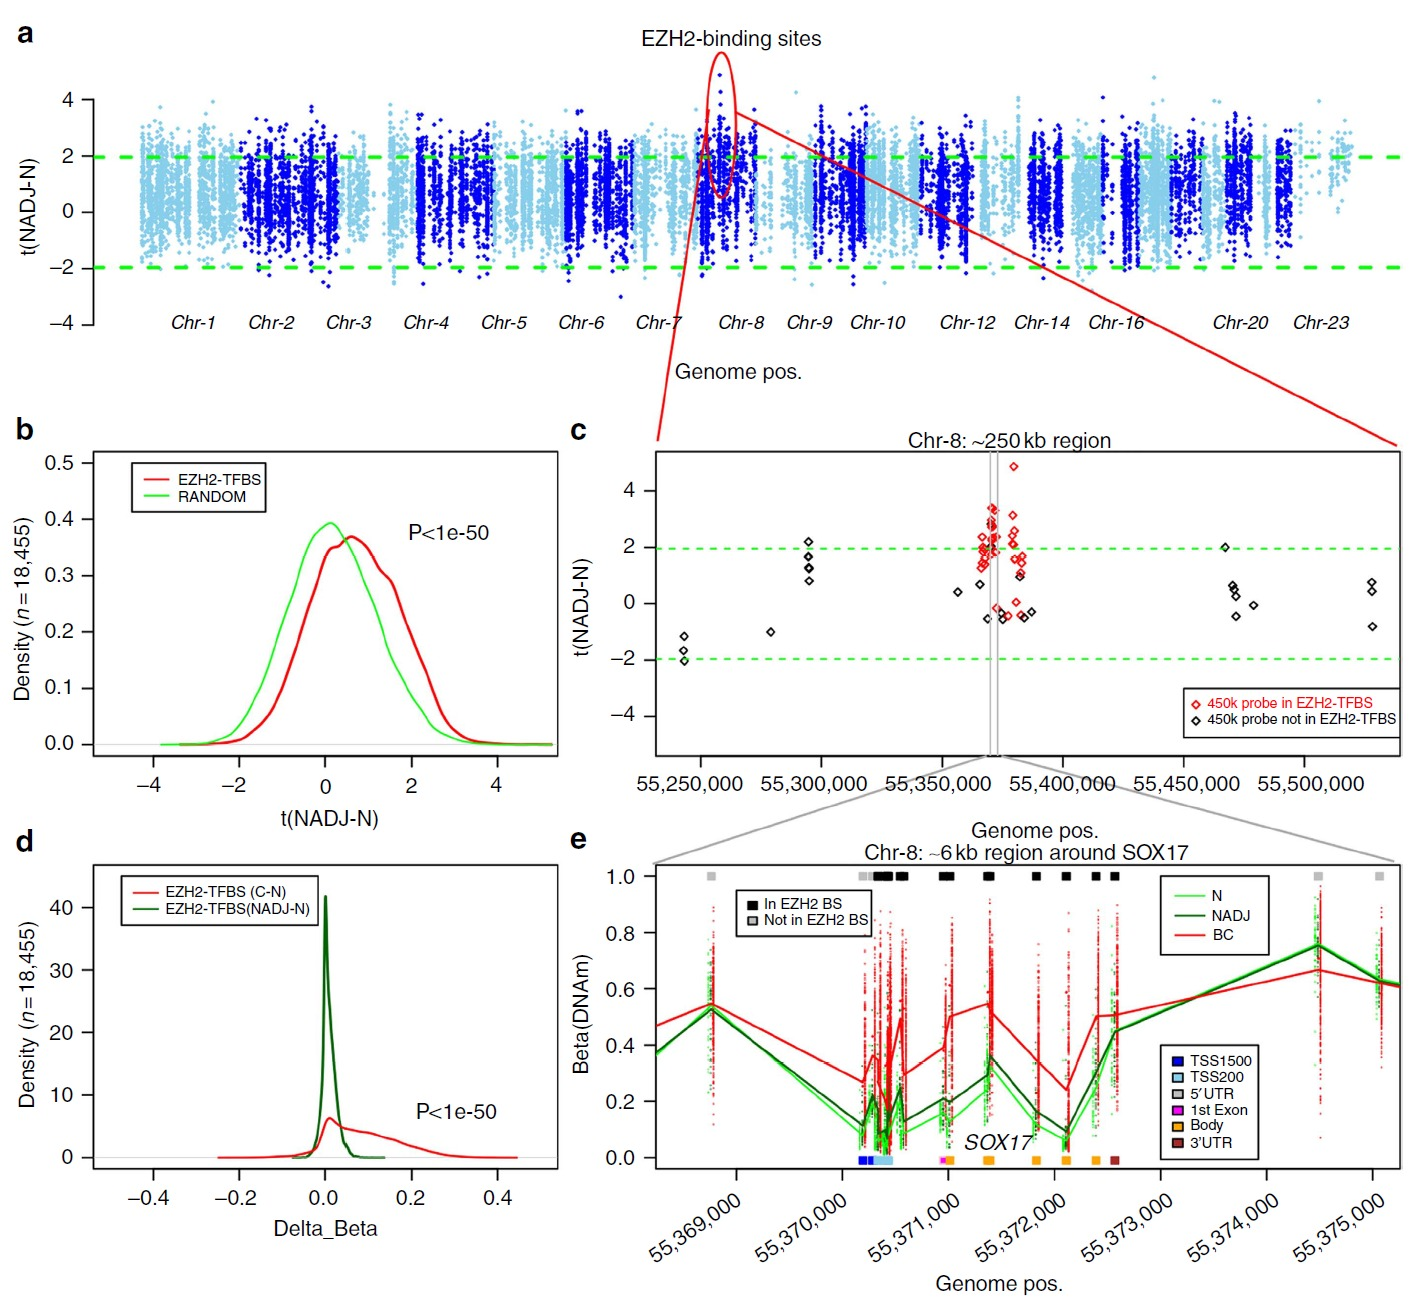
\includegraphics[width=0.5\textwidth]{Figures/Enrichment of EZH2 TF-binding sites among DNA methylation field defects..jpg} % o .png, .pdf, .eps...
    \caption{EZH2-associated DNA methylation patterns
CpG probes located within EZH2-binding sites show consistent hypermethylation in normal-adjacent breast tissue compared with normal tissue, indicating early Polycomb-associated epigenetic changes. The density and regional plots reveal a gradual methylation increase along the normal → adjacent → cancer sequence, exemplified by the \textit{SOX17} locus, where EZH2-bound CpGs gain methylation progressively. These patterns suggest that PRC2 targets undergo early and coordinated epigenetic activation preceding tumor development.}
    \label{fig:DNA_methylation_patters}
\end{figure}


\section{DNA Methylation Patterns in Normal Tissue Correlate more Strongly with Breast Cancer Status than Copy-Number Variants}

\paragraph{Keywords}
DNA methylation, copy-number variants (CNVs), breast cancer, epigenetic field defects, iEVORA algorithm, EpiDISH, cell-type deconvolution, GSE67919, GSE69914, risk prediction~\cite{gao2018dnamethylation}.

\paragraph{Study objectives}
Gao, Widschwendter and Teschendorff (2018) investigated whether epigenetic or genetic alterations in normal breast tissue are more predictive of cancer risk. Specifically, they compared the ability of DNA methylation (DNAm) and copy-number variation (CNV) profiles—obtained from the same Illumina HumanMethylation450K arrays—to discriminate between \textbf{normal-healthy}, \textbf{normal-adjacent to tumor}, and \textbf{cancerous} breast samples. The analysis aimed to test whether DNAm changes in the normal epithelium better reflect cancer field defects than CNV alterations.

\paragraph{Datasets and preprocessing}
Two independent breast tissue cohorts were analyzed:
\begin{itemize}[label=-]
\item The \textbf{Erlangen cohort}: 50 normal-healthy, 42 normal-adjacent, and 305 breast cancers, profiled on the Illumina 450K array.
\item The \textbf{Validation cohort (GSE67919)}: 18 normal-healthy (from reduction mammoplasty) and 70 normal-adjacent samples.
\end{itemize}
Data normalization and background correction were performed using the \texttt{minfi} R package. CNV inference was derived directly from methylation signal intensities using the \texttt{conumee} package, ensuring both methylation and copy-number profiles were obtained from identical assays, avoiding batch effects.

\paragraph{Cell-type deconvolution and reference construction}
Given the cellular heterogeneity of breast tissue (epithelial, adipose, immune), the authors built a reference DNAm database of 349 CpGs discriminating nine major cell types (epithelial, adipocytes, and seven immune subtypes). The reference was validated using:
(i) independent datasets (ENCODE, Blueprint), 
(ii) in-silico mixed cell populations, and 
(iii) purified cell samples.  
Using this reference, the \textbf{EpiDISH algorithm} estimated epithelial, adipose, and immune-cell fractions for each sample. This correction allowed methylation changes to be attributed to true epithelial alterations rather than cell composition shifts.

\paragraph{Identification of differentially variable CpGs (DVMCs)}
To detect epigenetic field defects, the authors applied their \textbf{iEVORA algorithm}, designed to identify CpGs with differential variance rather than mean-level differences. Between normal-healthy and normal-adjacent tissues:
\begin{itemize}[label=-]
\item CpGs with significant differential variance (FDR $< 0.001$, Bartlett’s test) and mean difference ($p < 0.05$, t-test) were selected as \textbf{differentially variable and methylated CpGs (DVMCs)}.
\item The majority showed increased variance (“hyperV DVMCs”) in normal-adjacent samples, suggesting stochastic epigenetic deregulation in tissue at risk.
\end{itemize}
HyperV DVMCs were confirmed to be independent of cell-type fraction changes and to localize preferentially within epithelial genomic regions, indicating that they reflect true epigenetic instability rather than compositional artifacts.

\paragraph{CNV calling and comparative analysis}
CNV profiles were inferred using \texttt{conumee}, followed by segmentation via circular binary segmentation (CBS). Copy-number states (gain/loss) were determined with adaptive, sample-specific thresholds accounting for stromal contamination.  
Differential CN analysis between normal and normal-adjacent tissue revealed no genome-wide significant differences; only marginal gains were detected. While 2,845 genes exhibited CN changes exclusively in normal-adjacent samples, these alterations were weaker and less consistent than methylation changes. Both CN and DNAm alterations were enriched in the matched cancers, but only DNAm patterns were strong enough to separate tissue classes.

\paragraph{Risk prediction and model validation}
Cancer risk predictors were trained independently on DNAm and CNV features using five-fold cross-validation and an adaptive-index algorithm:
\begin{itemize}[label=-]
\item \textbf{DNAm-based classifier}: achieved AUC = 0.94 (95\% CI: 0.88–1.0) in the discovery set and AUC = 0.84 (0.74–0.94) in the validation cohort (GSE67919).
\item \textbf{CNV-based classifier}: failed to discriminate normal vs. normal-adjacent tissue (AUC = 0.60 and 0.50, respectively).
\end{itemize}
Alternative CNV-calling pipelines (\texttt{cnAnalysis450k}, bin-level analysis, probe-level Elastic Net classifiers) confirmed the poor predictive performance of CNVs, indicating that the observed differences were not due to technical segmentation bias but reflect a genuine biological contrast.

\paragraph{Interpretation and implications}
DNAm alterations in normal-adjacent tissue mirror early “field defects” that are propagated and intensified in corresponding cancers. In contrast, CNVs—though enriched in tumors—show no significant discriminative power at the pre-cancer stage. The authors conclude that \textbf{epigenetic variability in normal cells better captures early carcinogenic processes} and thus provides a more sensitive predictor of breast cancer risk.  
The identified hyperV DVMCs often overlap with Polycomb (PRC2) target regions and developmental transcription factor binding sites, suggesting that aberrant methylation at these loci represents an early, reversible step toward neoplastic transformation.

\paragraph{Conclusion}
This work provides quantitative evidence that DNA methylation changes in histologically normal tissue are more predictive of cancer risk than copy-number variations. The methodological framework—EpiDISH correction, iEVORA feature selection, and risk-score modeling—demonstrates a reproducible way to extract early epigenetic markers from array data (e.g., GSE67919, GSE69914). The findings support a model where epigenetic instability precedes and possibly drives genetic alterations during tumor initiation.

\section{Large-scale analysis of DFNA5 methylation reveals its potential as biomarker for breast cancer}

\paragraph{Keywords}
DFNA5, breast cancer, DNA methylation, Illumina HumanMethylation450K, CpG biomarkers, logistic regression, AUC, survival, TCGA, ER status, ductal vs.\ lobular, prognostic markers~\cite{croes2018dfna5}.

\paragraph{Study design and datasets}
This study used The Cancer Genome Atlas (TCGA) to perform a large-scale, locus-specific analysis of DNA methylation in the \textit{DFNA5} (also known as \textit{GSDME}) gene in breast cancer. Only female, untreated, ductal or lobular breast adenocarcinoma samples were included. Methylation data were available for 668 primary breast adenocarcinomas and 85 histologically normal breast tissues sampled at a distance from the tumor; 79 of these patients had matched tumor/normal pairs. Expression data were available for 476 tumors and 56 normals (Agilent microarray) and 666 tumors and 71 normals (RNA-seq). Clinical parameters were collected for each patient: estrogen receptor (ER) status, progesterone receptor (PR) status, HER2 status, histological type (ductal vs.\ lobular), pathological tumor stage (I--IV), age at diagnosis, and overall survival (OS) up to 5 years after diagnosis. Three independent public datasets (GEO: GSE52865, GSE69914, GSE60185) were later used to externally validate classifier performance.

\paragraph{Methylation and expression profiling}
Genome-wide DNA methylation profiles were obtained from TCGA level-3 Illumina HumanMethylation450K BeadChip data. For \textit{DFNA5}, 22 distinct CpG loci on chromosome~7 were available. Methylation at each CpG was represented as a $\beta$ value, defined as the ratio of methylated probe intensity to the total probe intensity (methylated + unmethylated). Gene expression of \textit{DFNA5} was quantified using Agilent microarray and RNA-seq data, normalized as $\log_2$ fold-changes or abundance. Only 5 of 570 sequenced breast adenocarcinomas carried \textit{DFNA5} variants (3 missense, 2 silent), indicating that \textit{DFNA5} is rarely mutated; therefore, analysis focused on epigenetic regulation.

\paragraph{Statistical framework}
All statistical analyses were performed in \texttt{R}. Linear mixed models with batch as random effect and age as covariate were used for methylation/expression associations. For paired tumor/normal comparisons, paired $t$-tests were used. Stepwise logistic regression with tenfold cross-validation identified CpGs that best discriminated tumor from normal tissues, optimizing the area under the ROC curve (AUC). Cox proportional hazards models assessed whether CpGs contributed to 5-year OS prediction beyond age and tumor stage.

\paragraph{DFNA5 methylation landscape}
The 22 CpGs were distributed as follows:
\begin{itemize}[label=-]
\item \textbf{Gene body (6 CpGs):} CpG17790129, CpG14205998, CpG04317854, CpG12922093, CpG17569154, CpG19260663.
\item \textbf{Promoter region (14 CpGs):} CpG09333471, CpG00473134, CpG03995857, CpG07320646, CpG07293520, CpG04770504, CpG24805239, CpG01733570, CpG25723149, CpG22804000, CpG07504598, CpG15037663, CpG19706795, CpG20764575.
\item \textbf{Upstream region (2 CpGs):} CpG06301139, CpG26712096.
\end{itemize}
Breast cancers displayed clear promoter hypermethylation and gene-body hypomethylation. In the promoter, tumor $\beta$-values ranged 0.6–0.75 vs.\ 0.3–0.4 in normal tissue, while gene-body CpGs showed the opposite pattern (hypomethylation in tumor). These results indicate focal hypermethylation of regulatory regions concurrent with hypomethylation of coding regions.

\paragraph{Relationship between methylation and expression}
Tumors exhibited both promoter hypermethylation and lower \textit{DFNA5} expression compared with normal tissue, but direct CpG–expression correlations were modest ($|\rho|<0.35$). Multivariate models explained about 20\% of expression variance in tumors, suggesting methylation partially controls gene repression. This partial correlation may reflect tumor heterogeneity and the complex regulation of \textit{DFNA5} transcription.

\paragraph{Diagnostic classifier}
Stepwise logistic regression identified two CpGs that maximized tumor/normal discrimination:
\begin{itemize}[label=-]
\item \textbf{CpG12922093} (gene body, hypomethylated in tumor),
\item \textbf{CpG07504598} (promoter, hypermethylated in tumor).
\end{itemize}
The logistic model:
\[
\text{Pr}(\text{tumor}) = \frac{e^{7.49 - 10.77 \beta(\text{CpG12922093}) + 6.33 \beta(\text{CpG07504598})}}{1 + e^{7.49 - 10.77 \beta(\text{CpG12922093}) + 6.33 \beta(\text{CpG07504598})}}
\]
yielded tenfold cross-validated AUC = 0.93 (95\% CI: 0.92–0.95). Using a cutoff of 0.87 achieved 85.3\% sensitivity and 100\% specificity (accuracy 87\%). The model replicated well in GSE52865, GSE69914, and GSE60185 datasets. In contrast, \textit{DFNA5} expression alone provided lower AUCs (0.82–0.88), confirming methylation as a superior diagnostic marker.

\paragraph{Clinicopathological correlations}
\begin{itemize}[label=-]
\item \textbf{ER status:} Promoter CpGs were more methylated in ER$^+$ tumors, gene-body CpGs less methylated. \textit{DFNA5} expression was lower in ER$^+$ cancers.
\item \textbf{PR status:} 15 CpGs correlated with PR status, but expression differences were not significant.
\item \textbf{HER2 status:} Only CpG04317854 associated with HER2; expression unaffected.
\item \textbf{Tumor stage:} Five CpGs showed significant stage correlation.
\item \textbf{Histology:} Lobular carcinomas had higher promoter methylation (10 CpGs) and higher \textit{DFNA5} expression than ductal carcinomas, suggesting subtype-specific regulation.
\end{itemize}

\paragraph{Prognostic relevance}
Cox models revealed that five \textbf{gene-body CpGs}—CpG17790129, CpG14205998, CpG12922093, CpG17569154, and CpG19260663—were significantly associated with 5-year OS ($p<0.05$). Higher methylation at these loci predicted worse prognosis independently of stage and age. Promoter CpGs, while diagnostic, were not prognostic. Hence, promoter methylation primarily distinguishes tumors, while gene-body methylation predicts aggressiveness.

\paragraph{Replication protocol}
To reproduce these findings:
\begin{enumerate}
\item Extract $\beta$-values for the 22 CpGs from 450K data (TCGA or GEO).
\item Perform paired $t$-tests for tumor vs.\ normal and visualize mean $\beta$ by genomic position.
\item Fit logistic regression with all 22 CpGs; select the 2-CpG model above for classification.
\item Validate AUC through cross-validation or on external datasets (expected $\text{AUC}\approx0.93$).
\item Associate CpG methylation with ER, PR, HER2, histology using linear mixed models.
\item Fit Cox models for OS; expect significant gene-body CpG effects on prognosis.
\end{enumerate}

\paragraph{Conclusion}
Croes et al.\ demonstrated that \textit{DFNA5} promoter hypermethylation and gene-body hypomethylation constitute a reproducible epigenetic signature in breast cancer. The 22 CpGs identified delineate functional regions with diagnostic and prognostic value. The 2-CpG logistic model (CpG12922093, CpG07504598) offers a compact, high-specificity classifier (AUC = 0.93). Gene-body methylation correlates with poor prognosis, suggesting that \textit{DFNA5} methylation captures both tumor presence and aggressiveness. These results position \textit{DFNA5} as a promising epigenetic biomarker for breast cancer detection and risk stratification.

\begin{figure}[H]
    \centering
    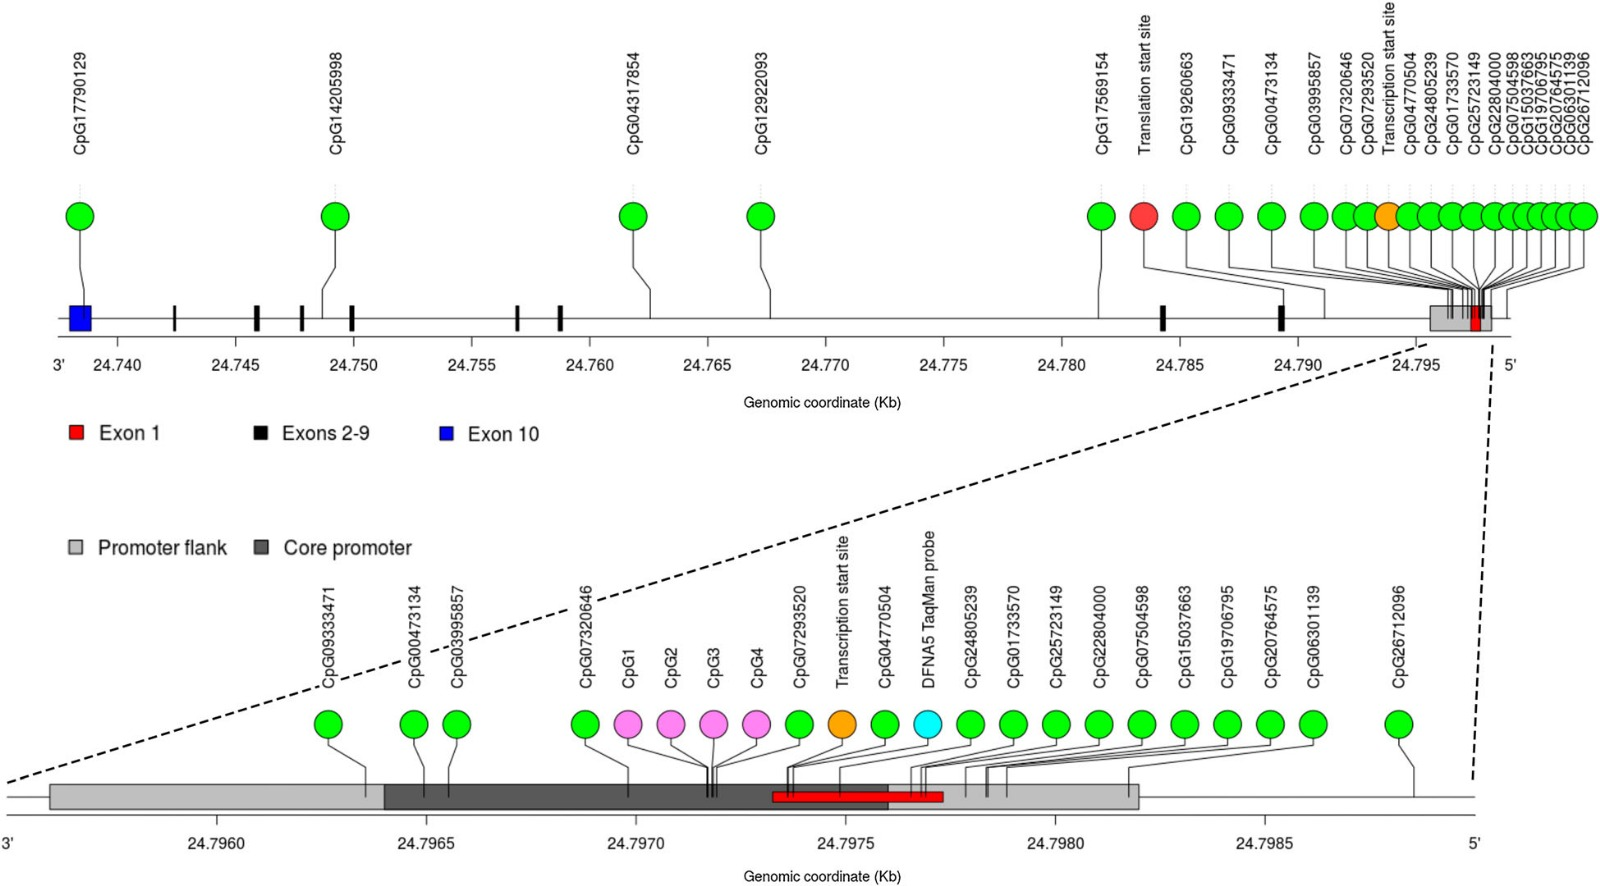
\includegraphics[width=0.7\textwidth]{Figures/The DFNA5 gene with annotation of the 22 CpGs..jpg} % o .png, .pdf, .eps...
    \caption{The DFNA5 gene with annotation of the 22 CpGs. The 10 exons and the promoter and gene body region of the DFNA5 gene are indicated.}
    \label{fig:22CpG}
\end{figure}


\section{Integrative analysis identifies potential DNA methylation biomarkers for pan-cancer diagnosis and prognosis}

\paragraph{Keywords}
DNA methylation, pan-cancer analysis, CpG biomarkers, TCGA, XGBoost, logistic regression, diagnostic classifier, prognostic model, differential methylation, feature selection, GSE69914~\cite{ding2019pancancer}.

\paragraph{Study design and objectives}
This large-scale integrative study aimed to identify CpG-based DNA methylation biomarkers with diagnostic and prognostic potential across multiple cancer types. The authors systematically analyzed genome-wide methylation data from 26 cancer types in The Cancer Genome Atlas (TCGA), covering 9,685 tumor samples and 729 matched normal tissues. The central goal was to develop a minimal CpG signature able to accurately (i) distinguish tumors from normal samples across cancers, (ii) identify the tissue of origin, and (iii) predict patient prognosis.

\paragraph{Data preprocessing and feature selection}
DNA methylation $\beta$-values (Illumina HumanMethylation450K array) were retrieved from TCGA. CpG probes with missing values in more than 20\% of samples or low variance ($\sigma^2 < 0.01$) were removed, leaving approximately 350,000 high-quality CpGs. Batch effects were minimized through quantile normalization and cross-cancer scaling of $\beta$-values to the [0,1] range.  
For each cancer type, differentially methylated CpGs (DMCs) were identified using a two-sided $t$-test comparing tumor vs. normal samples, controlling false discovery rate (FDR $<0.05$) and $|\Delta\beta| > 0.2$. These DMCs were pooled across cancers to obtain a global candidate set of $\sim$3,500 CpGs, which served as input for model training.

\paragraph{Diagnostic model construction (XGBoost + logistic regression)}
An extreme gradient boosting (\textbf{XGBoost}) model was used for feature selection to capture non-linear relationships among CpG methylation levels. The dataset was split into training (70\%) and testing (30\%) sets while maintaining cancer type stratification. Each CpG feature was assigned an importance score based on gain and coverage metrics from XGBoost iterations.  
The top 30 CpGs with the highest feature importance were retained, and a multivariate \textbf{logistic regression classifier} was trained on their $\beta$-values. Recursive feature elimination was then applied to minimize redundancy, resulting in a final diagnostic signature of \textbf{seven CpGs}.  
These seven CpGs achieved an average area under the ROC curve (AUC) of 0.982 in 10-fold cross-validation, and above 0.95 in nine independent cancer cohorts. Validation was also conducted on external GEO datasets, including breast tissue datasets such as GSE69914 and GSE76938, confirming the robustness of the selected CpGs across platforms.

\paragraph{Functional and genomic annotation of the 7 CpGs} These 7 CpGs function as a universal “epigenetic fingerprint” that clearly separates the methylation profiles of healthy tissues from those of tumors.
The 7 CpG sites are distributed across genes involved in tumorigenesis and transcriptional regulation:
\begin{itemize}[label=-]
\item \textbf{cg08244313 (ANKRD11)} – located in the promoter of a chromatin remodeling gene frequently mutated in breast and lung cancer; hypermethylation leads to transcriptional silencing and impaired cell differentiation.
\item \textbf{cg17735539 (ZNF582)} – located in a zinc-finger transcription factor promoter; hypermethylation is recurrent in cervical, colon, and breast cancers, acting as a universal tumor suppressor marker.
\item \textbf{cg21361244 (TRIM15)} – associated with ubiquitin-mediated protein degradation; its hypomethylation correlates with higher expression in invasive tumors.
\item \textbf{cg26157345 (CCDC181)} – localized in the gene body of a microtubule-associated protein; consistent hypermethylation across epithelial cancers suggests a pan-epithelial marker.
\item \textbf{cg11510243 (PDLIM4)} – involved in cytoskeletal anchoring and tumor suppression; promoter hypermethylation represses expression and promotes migration and metastasis.
\item \textbf{cg12542207 (SPG20)} – regulates cell cycle and WNT signaling; hypermethylated in multiple carcinomas, including breast, liver, and colon.
\item \textbf{cg18081940 (ZSCAN18)} – zinc-finger transcription regulator; hypermethylated in breast and endometrial cancers, associated with chromatin repression and proliferation.
\end{itemize}
Collectively, these CpGs represent \textbf{pan-cancer epigenetic switches} targeting genes involved in chromatin regulation, cytoskeletal integrity, and transcriptional control—biological processes frequently altered in early tumorigenesis. Their hypermethylation consistently marks the transition from normal to malignant epigenetic states.

\paragraph{Model validation and cross-cancer generalization}
To evaluate generalizability, the seven-CpG classifier was tested on unseen TCGA cancers (e.g., prostate, ovarian, kidney, brain). All achieved diagnostic AUC $>$ 0.97, confirming that the same CpG panel discriminates tumors from normals regardless of tissue origin.  
Moreover, an extended classifier including 12 additional CpGs was trained to predict cancer type (i.e., tissue of origin). This model achieved a macro-AUC of 0.95 across 26 TCGA cancers, correctly classifying both primary and metastatic samples in over 90\% of cases. The consistency of CpG methylation patterns across datasets and tissues underscores the universality of these epigenetic changes.

\paragraph{Prognostic analysis}
To assess survival relevance, patients were divided into high- and low-risk groups based on their mean methylation at the seven diagnostic CpGs. Kaplan–Meier and Cox proportional hazards analyses revealed that higher methylation of these CpGs correlated with shorter overall survival in seven cancer types, notably in breast, colon, and lung cancers (log-rank $p < 0.001$). The prognostic classifier demonstrated stable performance across cohorts, indicating that CpG methylation at these loci reflects tumor aggressiveness and progression dynamics.

\paragraph{Interpretation and reproducibility}
The seven identified CpGs form a minimal yet highly predictive signature of cancer-specific methylation. Their diagnostic capacity stems from consistent hypermethylation of regulatory promoters and transcription factor binding regions across epithelial cancers. Importantly, these CpGs can be measured on the Illumina 450K or EPIC arrays, allowing direct replication in datasets such as GSE69914. The pipeline—DMC selection, XGBoost feature ranking, logistic regression training, and ROC-based validation—offers a reproducible framework for building multi-cancer methylation classifiers.

\paragraph{Conclusion}
This integrative analysis demonstrates that DNA methylation profiling can yield robust, universal biomarkers for cancer detection and prognosis. The seven CpGs identified by Ding et al. serve as a compact and biologically interpretable panel capturing core epigenetic alterations across multiple tumor types. Their consistent hypermethylation patterns make them ideal candidates for clinical diagnostic assays and for cross-dataset validation in studies such as the present thesis.


\begin{figure}[H]
    \centering
    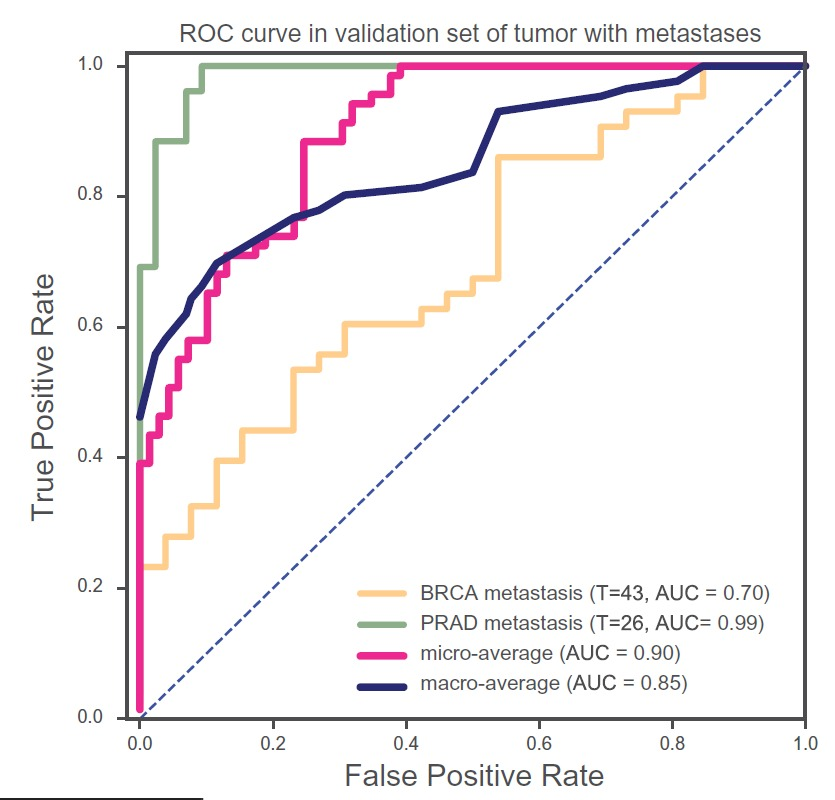
\includegraphics[width=0.3\textwidth]{Figures/Validation of tumor specific classifier in tumors with metastases.jpg} % o .png, .pdf, .eps...
    \caption{Validation of tumor specific classifier in tumors with metastases. ROC curve of multiclass tumor specific classifier in
metastatic breast cancer (GSE58999) and metastatic prostate cancer (GSE73549 and GSE38240).}
    \label{fig:ROC}
\end{figure}


\section{Prediction of Disease Genes Based on Stage-Specific Gene Regulatory Networks in Breast Cancer}

\paragraph{Keywords}
Breast cancer, DNA methylation, gene expression, stage-specific analysis, gene regulatory networks, WGCNA, hub genes, TCGA, GSE69914, GSE15852, candidate driver genes~\cite{fan2021stagegrn}.

\paragraph{Study aim and rationale}
This study proposes a computational framework to predict \textit{stage-specific} candidate disease genes in breast cancer by integrating transcriptomic and DNA methylation data with clinical staging information. Unlike many previous approaches that ignore stage and analyze tumors as a single group, this method builds three distinct regulatory models for Stage~I, Stage~II, and Stage~III breast cancer. The central idea is that genes driving cancer initiation may differ from those driving progression, and therefore network structure and key regulators should be inferred separately at each tumor stage. The pipeline identifies stage-specific gene modules, characterizes their biological functions, and prioritizes their core genes as putative disease genes for that stage. The approach is then validated on external datasets (GSE15852 and GSE69914) to assess reproducibility.

\paragraph{Datasets and preprocessing}
Gene expression (RNA-Seq) and DNA methylation data were downloaded from The Cancer Genome Atlas (TCGA), together with phenotype and staging data. The gene expression matrix contained 60{,}484 genes across 1{,}217 samples; the DNA methylation matrix contained 485{,}578 CpG sites across 890 samples. Only paired samples (each tumor sample matched to its own adjacent normal tissue) were retained. Samples were then stratified by clinical stage, yielding: 29 tumor/normal pairs for Stage~I, 94 pairs for Stage~II, and 32 pairs for Stage~III. Stage~IV had only two usable pairs and was excluded as not statistically convincing.

For methylation, multiple CpG probes can map to the same gene. The authors collapsed CpG-level data to gene-level methylation by averaging the $\beta$ values of all CpGs annotated to that gene. The $\beta$-value represents the methylation level; values $>0.8$ defined hypermethylated genes and values $<0.2$ defined hypomethylated genes.

For gene expression, normalized FPKM values were used. Genes with missing values in more than 15\% of samples were filtered out. Only those samples with both gene expression and matched methylation data (tumor and normal from the same patient) were kept for downstream paired analyses.

\paragraph{Differential expression and methylation filtering}
Within each stage separately (Stage~I, Stage~II, Stage~III), tumor vs.\ matched normal samples were compared to identify both (i) differentially expressed genes and (ii) aberrantly methylated genes.

Differential expression analysis was performed using the \texttt{limma} R package, selecting genes with $p<0.05$ and $|\log \text{FC}|<0.5$ as reported thresholds. In parallel, DNA methylation status was used to label genes as hypermethylated ($\beta > 0.8$) or hypomethylated ($\beta < 0.2$). The intersection of these two criteria --- genes that were both differentially expressed and abnormally methylated --- produced the gene sets carried forward for network modeling. This yielded 1{,}027 such genes in Stage~I, 1{,}012 in Stage~II, and 1{,}220 in Stage~III.

Across all stages, the authors confirmed the expected inverse relationship between DNA methylation and gene expression: higher methylation corresponded to lower expression, consistent with promoter silencing effects.

\paragraph{Stage-specific gene regulatory network construction}
To model regulatory control at each stage, the study built three transcriptional regulatory networks (one per stage). Transcription factor (TF) $\rightarrow$ target gene pairs were obtained from GRNdb, a curated TF--target interaction resource. These TF--target pairs were filtered so that the target gene was among the stage-specific differentially expressed and hyper/hypomethylated genes defined above.

For each retained TF--target pair, the Pearson correlation coefficient (PCC) between TF expression and target expression was computed across the paired tumor/normal samples of that stage. Edges with $|\text{PCC}| \ge 0.5$ were kept. This procedure produced three \textbf{stage-specific gene regulatory networks:}
\begin{itemize}[label=-]
    \item Stage~I network: 1{,}129 nodes and 4{,}429 edges.
    \item Stage~II network: 1{,}066 nodes and 4{,}879 edges.
    \item Stage~III network: 1{,}339 nodes and 6{,}461 edges.
\end{itemize}
These per-stage networks reflect transcriptional wiring specific to that disease stage, integrating both expression deregulation and methylation dysregulation relative to normal tissue.

\paragraph{Module detection via WGCNA}
Within each stage-specific regulatory network, modules (i.e., co-regulated and co-expressed gene communities) were identified using Weighted Gene Co-expression Network Analysis (WGCNA). The steps were: (i) hierarchical clustering of genes in each network; (ii) Dynamic Tree Cut to segment the dendrogram into discrete modules, enforcing a minimum module size of 30 genes.

Results:
\begin{itemize}[label=-]
    \item Stage~I network was partitioned into 11 modules (e.g., S1\_turquoise, S1\_brown, S1\_blue), with the largest (S1\_turquoise) containing 270 genes.
    \item Stage~II network was partitioned into 10 modules, with the largest (S2\_turquoise) containing 337 genes.
    \item Stage~III network was partitioned into 13 modules, with the largest (S3\_turquoise) again containing 337 genes.
\end{itemize}

Genes that were differentially expressed \textit{only} in one stage (not in the others) were labeled as ``stage-specific genes'': 92 genes for Stage~I, 60 for Stage~II, and 187 for Stage~III. The authors then mapped these uniquely stage-specific genes back to the WGCNA modules to identify which modules were most enriched for stage-unique signals. They found:
\begin{itemize}[label=-]
    \item Stage~I-specific genes mainly cluster in S1\_brown, S1\_turquoise, and S1\_blue.
    \item Stage~II-specific genes mainly cluster in S2\_turquoise.
    \item Stage~III-specific genes mainly cluster in S3\_turquoise, S3\_brown, and S3\_green.
\end{itemize}

These seven modules (S1\_brown, S1\_turquoise, S1\_blue, S2\_turquoise, S3\_turquoise, S3\_brown, S3\_green) were therefore defined as the \textbf{stage-specific core modules}.

\paragraph{Topological analysis of the core modules}
For each of the seven core modules, the study characterized network topology using Cytoscape. Metrics included node degree, betweenness centrality, and closeness centrality.

\begin{itemize}[label=-]
    \item Degree distributions in S1\_turquoise, S2\_turquoise, and S3\_turquoise were broad and extended to high connectivity: most node degrees lay between $\sim$100 and 400, implying dense regulatory connectivity in these ``turquoise'' modules.
    \item In S1\_brown, S1\_blue, S3\_brown, and S3\_green, degree values were generally lower (mostly 50--100) but still showed scale-free-like (power-law) behavior.
    \item Betweenness centrality was high for many nodes across all seven modules, and closeness centrality values for most nodes ranged from 0.5 to 0.9.
\end{itemize}

These metrics indicate that each stage-specific module is internally well connected, suggesting that its high-centrality nodes function as regulatory hubs. Such hubs are natural candidates for stage-relevant driver genes.

\paragraph{Functional enrichment of stage-specific modules}
Gene set enrichment analysis for each of the seven core modules was performed with Metascape, using a significance cutoff of $p<0.01$. The most significantly enriched biological themes were:
\begin{itemize}[label=-]
    \item \textbf{Cell cycle control and mitosis}: ``cell cycle phase transition,'' ``chromosome segregation,'' ``DNA replication,'' ``spindle organization,'' and ``cell division.'' These functions dominated the large turquoise modules of Stage~I, Stage~II, and Stage~III (S1\_turquoise, S2\_turquoise, S3\_turquoise).
    \item \textbf{Transcriptional regulation and chromatin state}: modules such as S1\_brown, S1\_blue, S3\_brown, and S3\_green were enriched for transcriptional activator/repressor activity, chromatin binding, histone modification, nuclear receptor activity, telomerase complex, and macromolecule methylation.
\end{itemize}

Importantly, regulatory complex assembly at promoters and chromatin binding functions were found across \textit{all} seven modules, suggesting that stage-specific dysregulation in breast cancer converges on control of transcription, chromatin structure, and cell cycle checkpoints.

\paragraph{Candidate disease gene prioritization}
Within each of the seven core modules, the authors defined ``core genes'' using two complementary strategies and then took their intersection:
\begin{enumerate}
    \item \textbf{Correlation structure within the module}: for each module, they computed a gene--gene correlation matrix and retained genes with correlation $\ge 0.8$ and $p<0.05$, marking them as internally coherent regulators.
    \item \textbf{Network centrality}: they ranked genes by degree, betweenness centrality, and closeness centrality within that module and selected the top 5\% as hub-like nodes.
\end{enumerate}

Genes that satisfied both criteria were labeled \textbf{candidate disease genes} for that stage.

Results by stage:
\begin{itemize}[label=-]
    \item \textbf{Stage~I} (modules S1\_brown, S1\_turquoise, S1\_blue): 20 candidate genes, including \textit{E2F2}, \textit{E2F8}, \textit{TPX2}, \textit{BUB1}, \textit{CKAP2L}, \textit{CBX3}, \textit{KPNA2}, \textit{NEK2}, \textit{TTK}, \textit{LMNB1}, \textit{SLC25A36}, \textit{SLC39A1}, \textit{MRPS12} (PCNA-related), and additional transcriptional/transport regulators like \textit{CASC5}, \textit{CREBRF}, \textit{PAN2}, \textit{BTAF1}, \textit{ZC3H6}, \textit{DDX49}.
    \item \textbf{Stage~II} (module S2\_turquoise): 12 candidate genes, including \textit{E2F2}, \textit{E2F8}, \textit{TPX2}, \textit{KPNA2}, \textit{CKAP2L}, \textit{CBX3}, \textit{BUB1}, \textit{CCNE2}, \textit{CASC5}, \textit{SPDL1}, \textit{TOP2A}, and \textit{DDIAS}.
    \item \textbf{Stage~III} (modules S3\_turquoise, S3\_brown, S3\_green): 22 candidate genes, including \textit{E2F2}, \textit{RAD21}, \textit{FBXO5}, \textit{CCNE2}, \textit{CBX3}, \textit{STIL}, \textit{CKAP2L}, \textit{PCNA}, \textit{NEK2}, \textit{TTK}, \textit{CSE1L}, \textit{H2AFZ}, \textit{NR2F6}, \textit{TRAPPC6A}, \textit{IGSF8}, \textit{FDXR}, \textit{SLC39A1}, \textit{EXOSC5}, \textit{RBBP5}, \textit{KDM5B}, \textit{H3F3A}, and \textit{CDC42SE1}.
\end{itemize}

Three genes --- \textit{E2F2}, \textit{CKAP2L}, and \textit{CBX3} --- were shared across all three stages, suggesting persistent dysregulation from early to late disease.

\paragraph{Biological/clinical interpretation and validation}
The candidate genes were then checked against known cancer gene resources (OMIM, COSMIC, DAVID) and literature in PubMed to test whether they are already associated with breast cancer biology.

Many top hits have clear functional relevance:
\begin{itemize}[label=-]
    \item \textit{E2F2}, \textit{E2F8}: transcription factors controlling cell cycle entry and proliferation; linked to poor prognosis and recurrence-free survival in breast cancer.
    \item \textit{TPX2}, \textit{BUB1}, \textit{NEK2}, \textit{TTK}, \textit{TOP2A}, \textit{PCNA}: mitotic spindle assembly, checkpoint control, DNA topology, and replication; these genes support uncontrolled proliferation and chromosomal instability.
    \item \textit{CKAP2L}, \textit{CASC5}, \textit{FBXO5}, \textit{STIL}: regulators of mitosis, centrosome function, or chromosomal segregation, repeatedly linked to aggressive tumor behavior and poor prognosis in breast cancer.
    \item \textit{RAD21}: DNA repair and chromosomal cohesion, implicated in therapy response.
    \item \textit{KDM5B}, \textit{CBX3}, \textit{H2AFZ}: chromatin and epigenetic regulators whose overexpression correlates with metastatic potential, proliferation, and reduced survival.
    \item \textit{CSE1L}, \textit{CCNE2}: associated with metastasis and poor clinical outcome in breast tumors.
\end{itemize}

Overall, 55\% of Stage~I candidates, 83\% of Stage~II candidates, and 64\% of Stage~III candidates were already supported by curated cancer resources or published studies as breast cancer--related. This high validation rate supports the predictive value of the stage-specific module approach.

\paragraph{External validation using independent datasets (GSE15852 and GSE69914)}
To further test generalizability, the authors reapplied their framework to two public GEO datasets:
\begin{itemize}[label=-]
    \item GSE15852: gene expression data from 43 primary breast cancers and their matched normal tissues.
    \item GSE69914: Illumina 450K DNA methylation data including paired normal-adjacent and tumor breast tissue samples.
\end{itemize}

From these datasets, they identified 79 genes that were both differentially expressed and aberrantly methylated. Using TF--target information and PCC~$\geq 0.5$, they built a combined breast cancer regulatory network with 195 nodes and 313 edges, then used WGCNA to divide it into modules (turquoise, blue, brown; gray genes were unassigned and discarded). Applying the same two-step prioritization (correlation $\geq 0.8$ with $p<0.05$ and top 5\% centrality), they obtained a focused set of 10 candidate genes: \textit{H2AFZ}, \textit{NPM1}, \textit{MAF}, \textit{NR3C1}, \textit{PTGER3}, \textit{TCF4}, \textit{IRF1}, \textit{RARB}, \textit{CHD2}, and \textit{SMAD4}. All but \textit{PTGER3} and \textit{CHD2} were previously linked to breast cancer biology or prognosis. This reproduced the core logic of the pipeline (methylation + expression + regulatory structure + module centrality) on independent data, including GSE69914, and again recovered biologically meaningful breast cancer genes.

\paragraph{Replication workflow for a new dataset}
The procedure described in this work can be replicated on any breast cancer dataset with (i) gene expression, (ii) DNA methylation, and (iii) clinical staging or at least tumor vs.\ matched normal pairs:
\begin{enumerate}
    \item \textbf{Stratify by stage}: split tumor/normal pairs into Stage~I, Stage~II, Stage~III (or other clinically defined strata). Exclude strata with too few matched pairs.
    \item \textbf{Call altered genes}: within each stage, find differentially expressed genes using \texttt{limma} with $p<0.05$ and $|\log \text{FC}|<0.5$ as stated; classify genes as hypermethylated ($\beta>0.8$) or hypomethylated ($\beta<0.2$). Take the intersection of these two sets to focus on genes that are both transcriptionally deregulated and epigenetically abnormal.
    \item \textbf{Build stage-specific TF$\to$target networks}: obtain TF--target pairs (e.g., from GRNdb), keep those whose targets are in the intersected gene list, and compute Pearson correlation between TF and target across that stage's samples. Retain edges with $|\text{PCC}|\ge 0.5$.
    \item \textbf{Detect co-regulated modules}: run WGCNA on each stage-specific network. Use hierarchical clustering + Dynamic Tree Cut, enforcing a minimum of $\sim$30 genes per module.
    \item \textbf{Identify ``core'' stage modules}: determine which modules are enriched for genes unique to that stage (i.e., differentially expressed only in Stage~I, only in Stage~II, etc.). These modules are considered the disease-relevant stage-specific modules.
    \item \textbf{Prioritize candidate disease genes}: within each stage-specific module, (a) keep genes with strong within-module correlation ($\ge 0.8$, $p<0.05$), and (b) keep the top 5\% highest-ranked genes by degree, betweenness centrality, and closeness centrality. The intersection are the candidate stage-specific disease genes.
    \item \textbf{Biological interpretation}: run functional enrichment (e.g., Metascape) to reveal dominant pathways (cell cycle, chromatin remodeling, spindle checkpoint, transcriptional control). Cross-reference the prioritized genes with OMIM, COSMIC, DAVID, and PubMed to evaluate known breast cancer relevance and prognostic value.
\end{enumerate}

\paragraph{Conclusion}
By integrating DNA methylation, gene expression, TF--target regulatory structure, and explicit stage information, this framework reveals modules of tightly connected, transcriptionally dysregulated, and epigenetically altered genes that are specific to Stage~I, Stage~II, or Stage~III breast cancer. These modules are enriched for cell cycle, chromatin regulation, mitotic checkpoint control, and transcriptional programs known to underlie tumor progression. The most central genes in these modules --- including \textit{E2F2}, \textit{E2F8}, \textit{TPX2}, \textit{BUB1}, \textit{CKAP2L}, \textit{CBX3}, \textit{RAD21}, \textit{CCNE2}, \textit{STIL}, \textit{KDM5B}, \textit{TOP2A}, \textit{PCNA} --- are strongly supported by literature as drivers of proliferation, chromosomal instability, epigenetic reprogramming, and metastatic potential in breast cancer. The method therefore provides a reproducible, stage-aware strategy to nominate disease genes and potential therapeutic targets, and it was shown to generalize to independent datasets including GSE69914.

\begin{figure}[H]
    \centering
    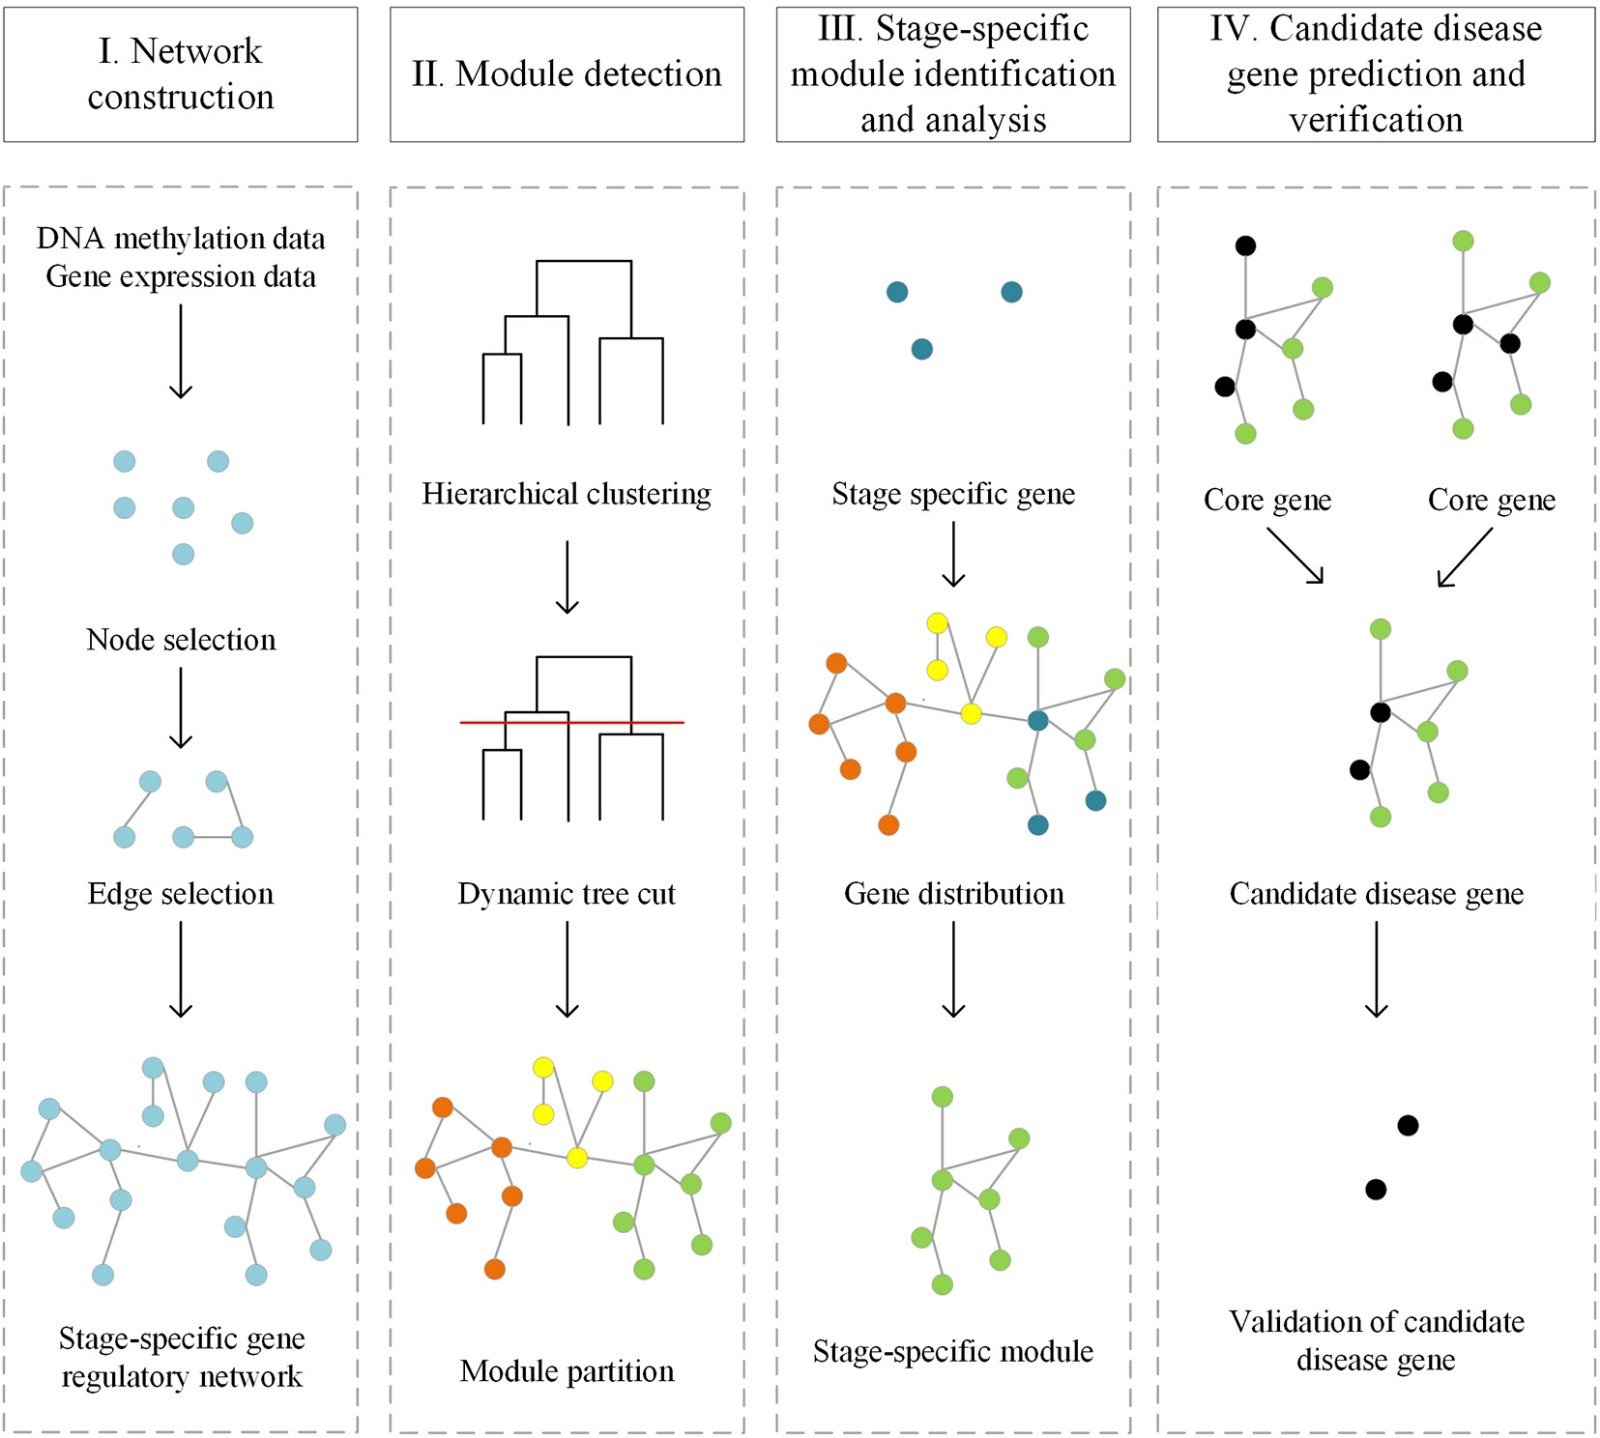
\includegraphics[width=0.6\textwidth]{Figures/Workflow of the computational framework for predicting disease genes based on stage-specific gene regulatory network.jpg} % o .png, .pdf, .eps...
    \caption{Workflow of the computational framework for predicting disease genes based on stage-specific gene regulatory network.}
    \label{fig:Workflow}
\end{figure}


\printbibliography
\end{document}
